\subsection{The XGBoost Tuner}

In TVM framework, \cite{Tianqi2018} proposed a configuration tuning method for operator-level optimization in which the search is guided by a performance prediction model trained with eXtreme Gradient Boosting (XGBoost). This XGBoost guided tuner (or XGBoost tuner) follows an iterative search process. In each iteration, a large number of configuration candidates are derived from configuration space by random walk. According to the predicted performance from a trained XGBoost model, the best candidates are selected and tested on hardware. The performance feedback from the hardware is collected and applied to further train the XGBoost model so as to improve its prediction accuracy.

The XGBoost tuner outperforms the other classic tuners including genetic algorithm search, random search, etc., for GEMM. Nevertheless, training the XGBoost model for a large configuration space would incur a high cost. In order to further improve the operator-level configuration tuning performance, we propose a new configuration search model which allows exploitation of relations between similar configurations, followed by two efficient tuning methods.


\subsection{Configuration Search Modeling}

For better analysis, we model the configuration tuning problem as a Markov Decision Process (MDP), where each configuration can be regarded as a unique state. We define the state as follows.

\begin{equation}
    s = \left[ s_m, s_k, s_n, J \right],
\end{equation}
where $s_m = \left[ m_0, m_1, \ldots, m_{d_m-1} \right] \in \xi_m$, $s_k = \left[ k_0, k_1, \ldots, k_{d_k-1} \right] \in \xi_k$, $s_n = \left[ n_0, n_1, \ldots, n_{d_n-1} \right] \in \xi_n$, and $J$ is the binary number indicating whether the state is legitimate (e.g. the product of $m_i$'s must be $m$, the numbers must be integers, etc.).

As in the GEMM application, with similar configuration settings, i.e., the configuration parameters for each dimension of two states are equal or close, the performance of this two states may not exists large difference. Taking advantage of the relations among similar configurations, and considering the constraints of the matrices size in each configuration. We define the concept of action space as follows.

\begin{equation}
    \mathcal{A} = \left[ \begin{array}{l}
         {s_x[i] = 2s_x[i] ~~\text{and}~~ s_x[j]=s_x[j]/2 }, \\ \\
         {\text{where}~ \forall x \in \{m,k,n\}, \forall i, j \in [0, d_x)~\text{and}~ i \neq j }
    \end{array}
     \right].
\end{equation}
Accordingly, we define a step function $step$, i.e.,
\begin{equation}\label{fun:stepfun}
    s'= step(s,a).
\end{equation}
With the input of any action $a \in \mathcal{A}$, the current state $s$ is transferred to state $s'$. We define $s$ and $s'$ are neighbor states. Based on the setting of action space, we guarantee the Euclidean distance between the neighbor state $s$ and $s'$ is the minimum value compared with the distance between the state $s$ and all the other states.

Moreover, in order to better evaluate the performance of each action based on different states, if the agent takes action $a$ and goes from the state $s$ to the state $s'$, we define the rewards as follows
\begin{equation}
    r(s,a) = \frac{1}{T_{cost}(s'; m,k,n,d_m,d_k,d_n) }.
\end{equation}

Following the above modeling, the agent is expected to determine its policy $\boldsymbol{\pi}$ so as to efficiently approach and discover the state $s^*$ with the lowest running time in hardware system. In the following subsections, we will analyze two different configuration tuning approaches guided by G-BFS and N-A2C reinforcement learning, followed by a discussion for their strengths with different scenarios.



\subsection{G-BFS Method}

\begin{figure*}
\centering
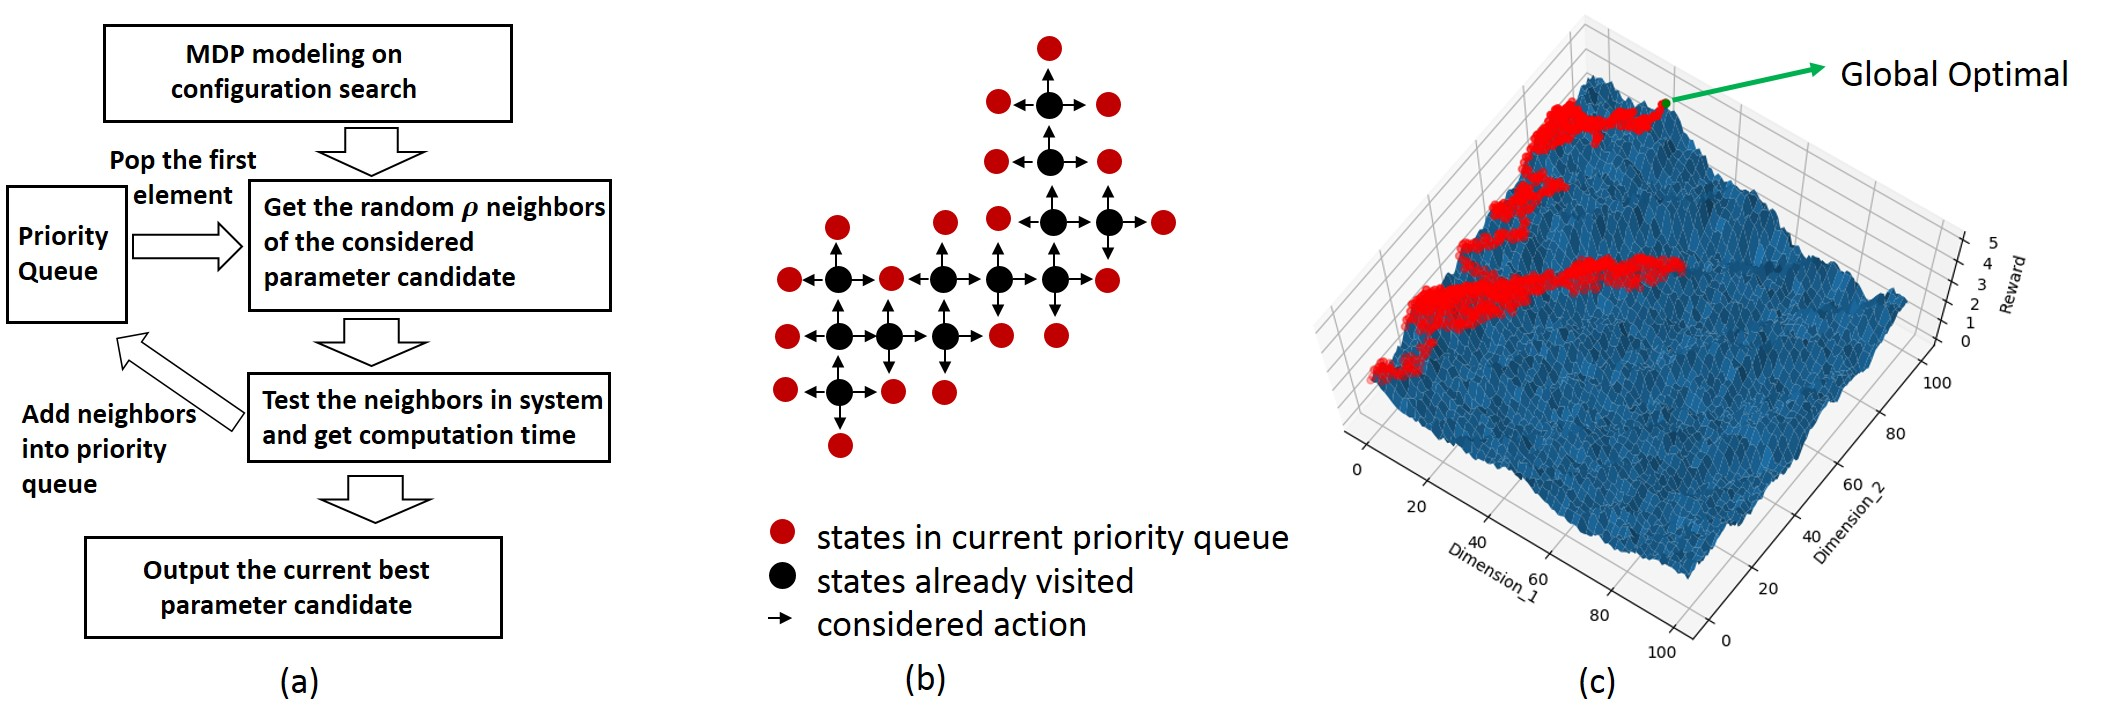
\includegraphics[scale=0.4]{4_Method/gbfs_pic.jpg}
\caption{G-BFS Method}
\label{fig:gbfs}
\end{figure*}

The G-BFS method is guided by Greedy Best-First-Search and follows the flowchart in Fig. \ref{fig:gbfs}(a). We initialize an empty priority queue $\mathcal{Q}$ (ordered by increasing cost), an empty list $S_v$ to record all visited configuration candidates, and a random or hand-crafted starting state $s_0$. We first test and enque the starting state $s_0$ and record its running time $T_{cost}(s_0)$ into the priority queue $Q$. Based on the configuration search model, for each iteration, we deque the top configuration candidate $s$ from the priority queue $Q$. We iterate through all actions $a\in \mathcal{A}$ and collect all corresponding neighbor states as
\begin{equation}
    g(s) = [s'=step(s,a) ~~ \forall a \in \mathcal{A}].
\end{equation}
We randomly select $\rho$ ($\rho \in \{1,2,\ldots,len(g(s)) \}$) configuration candidates from $g(s)$, and test them in hardware. For each state $s'$ sampled from $g(s)$, if state $s'$ is legitimate and has not been visited before, we enque state $s'$ and its tested running time $T_{cost}(s')$ into $Q$ and add state $s'$ in the visited list $S_v$. If its tested running time $T_{cost}(s')$ is smaller than the current minimum running time, we set state $s'$ as the optimal state visited and record its running time as $t_{cost}^{min}$. The iteration continues until the priority queue is empty or the computation time reaches the maximum time specified by the user. The current stored optimal state $s*$ and its running time $t_{cost}^{min}$ are returned as tuning results. The summary of the algorithm is shown in Algorithm \ref{alg:gbfs}.

In Fig. \ref{fig:gbfs}(b), we show the exploration situation in the middle of the tuning algorithm when $\rho = len(g(s))$, where the red nodes denote the state currently stored in the priority queue and the grey nodes are all the visited states. In future iterations, the method will explore from the current most promising red nodes expands its visited state areas. In Fig. \ref{fig:gbfs}(c), we take an example of 2-dimensional configuration search on the randomly generated rewards function. We discover that the proposed G-BFS method is able to correct itself from exploring wrong directions and efficiently expand its neighborhood to the optimal states. Moreover, when the value of $\rho = len(g(s))$, given unlimited tuning time, the algorithm is guaranteed to visit all the configuration states.

\begin{algorithm}[htb]
\caption{G-BFS Method}
\label{alg:gbfs}
\vspace{.1cm}
\hrule
    \begin{algorithmic}[1]
    \vspace{.2cm}
    \STATE Initialization: $\mathcal{Q}$=PriorityQueue(), $S_v$, $s_0$
    \STATE Q.push($(T_{cost}(s_0), s_0)$);\\
    \STATE Add $s_0$ in $S_v$;\\
    \WHILE{$Q\neq \O$ and $t<T^{max}$}
        \STATE $(T_{cost}(s), s)$ = Q.pop(); \\
        \STATE $\mathcal{B}_{test}$ = Sample $\rho$ randomly from $g(s)$; \\
        \FOR{$s'$ in sampled configuration candidates}
            \IF{$s'[-1]=True$ and $s' \not\in S_v$}
                \STATE Q.push($(T_{cost}(s'), s')$); \\
                \STATE Add $s'$ in $S_v$;\\
                \IF{$t_{cost}^{min} > T_{cost}(s')$}
                    \STATE $t_{cost}^{min} = T_{cost}(s')$; \\
                    \STATE $s^* = s'$;
                \ENDIF
            \ENDIF
        \ENDFOR
    \ENDWHILE
    \STATE Return: The optimal configuration $s^*$ with cost $t_{cost}^{min}$.
    \end{algorithmic}
\hrule
\end{algorithm}






\subsection{N-A2C Method}






\begin{algorithm}[htb]
\caption{N-A2C Method}
\label{alg:r_a2c}
\vspace{.01cm}
\hrule
    \begin{algorithmic}[1]
    \vspace{.2cm}
    \STATE Initialization: {$s_0$, $\mathcal{M}$, $H_v$}
    \FOR{each episode}
        \WHILE{$len(\mathcal{B}_{collect})< len(\mathcal{B}_{test})$ }
            \STATE$s = s_0$; \\
            \FOR{each step until $T$ steps}
                \IF{$rand()<\tau$}
                    \STATE $a$ follows $\pi(s)$;
                \ELSE
                    \STATE $a$ is random selected from $\mathcal{A}$;
                \ENDIF
                \STATE $s'=step(s,a)$; \\
                \IF {$s'$ not in $H_v$}
                    \STATE Add $s'$ in $\mathcal{B}_{collect}$;
                \ENDIF
                \STATE $s = s'$;
            \ENDFOR
        \ENDWHILE
        \FOR{$s'$ in $\mathcal{B}_{collect}$}   % Can be done in parallel computing
            \IF{$t_{cost}^{min} > T_{cost}(s')$}
                \STATE $t_{cost}^{min} = T_{cost}(s')$; \\
                \STATE $s^* = s'$; \\
                \STATE $s_0=s^*$; \\
            \ENDIF
            \STATE $H_v[s'] = T_{cost}(s')$; \\
            \STATE Store $(s, a, r(s,a), s')$ to $\mathcal{M}$, where $\forall s$, $\forall a$ satisfying $step(s,a) = s'$; \\
            \STATE Train actor's and critic's neural networks with $\mathcal{M}$;
        \ENDFOR
    \ENDFOR
    \STATE Return: The optimal configuration $s^*$ with cost $t_{cost}^{min}$.
    \end{algorithmic}
    \hrule
\end{algorithm}

As the G-BFS method explores only one step from the considered state for each iteration, its performance may be affected when the running time from similar states exhibits large random noise. In the N-A2C method, as shown in Fig. \ref{fig:r_a2c}(a), for each episode, we let the exploration being generated in a $\varsigma$-step neighborhood, and the direction of exploration is guided with A2C reinforcement learning method \cite{bhatnagar2009natural}. The center of the exploration neighborhood is periodically updated with the optimal states ever visited.


We summarize the tuning method in Algorithm~\ref{alg:r_a2c}. Initially, we set a random or experience-estimated starting state $s_0$, a fixed-size memory buffer $\mathcal{M}$ to record the latest searching information and an empty hashtable $H_v$ recording all the visited states with their running time. For the A2C reinforcement learning model, both actor and critic firstly establish their neural networks with random weights, respectively. Following the configuration search model, for each episode, while the collected configuration candidates for testing is less than the predefined tested batch size, iteratively, from the same starting point, the agent explore $\mathcal{T}$ continuous steps. For each step, with probability of $\tau$, the agent take action $a$ guided by the policy $\pi(s)$ from the actor's nerual network; With probability of $1-\tau$, the agent choose a random action $a$ from current state. Based on the current state $s$ and action $a$, we get the next state $s'$ from (\ref{fun:stepfun}). If the next state $s'$ has not been visited before, we add the state $s'$ in collected candidate batch $\mathcal{B}_{collect}$.




When the number of collected candidates $\mathcal{B}_{collect}$ achieve the predefined test size, we let the system run the collected configuration candidates. Based on the corresponding running time, the stored hashmap $H_v$ and memory buffer $\mathcal{M}$ is updated. Based on updated $\mathcal{M}$, by randomly selecting history exploration data, the neural networks of A2C reinforcement learning is trained.



Generally, the proposed N-A2C method is able to efficiently search the optimal GEMM configuration with fixed exploration step in each episode. Nevertheless, in order to find the most important exploration neighborhood, the exploration step $\mathcal{T}$ can have a soft start, which means starting with a large value and gradually reduce to a small number. Moreover, in order to fully explore the configuration space, after a long time exploration within the same starting points, the exploration step $\mathcal{T}$ will gradually increase to further explore new configuration candidates.

In Fig. \ref{fig:r_a2c}(b), we show a simple exploration map with the proposed N-A2C method. With more explorations, the exploration neighborhood changes with the update of optimal states ever visited. In Fig. \ref{fig:r_a2c}(c), we take an example of 2-dimensional configuration on the randomly generated rewards function. Due to the large randomness in the example, we set the exploration step $\mathcal{T}$ as 100 and the global optimal state can be efficiently discovered with the assistance of the A2C reinforcement learning algorithm.

\begin{figure*}
\centering
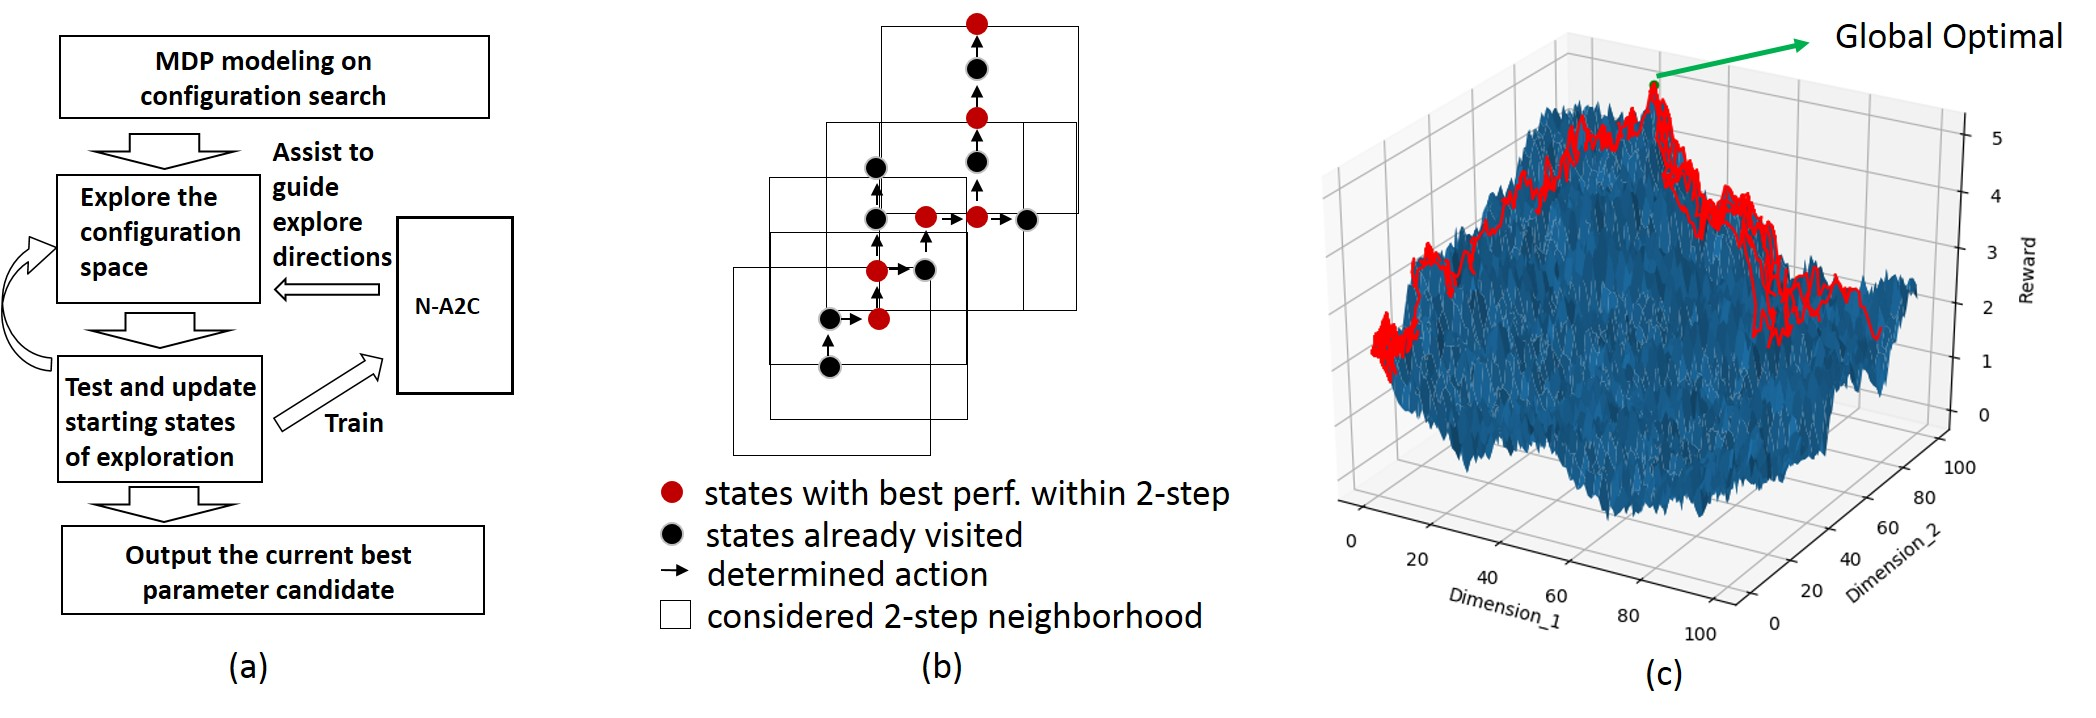
\includegraphics[scale=0.4]{4_Method/n_a2c_pic.jpg}
\caption{N-A2C Method}
\label{fig:r_a2c}
\end{figure*}


\subsection{Discussion}
We compare the G-BFS guided tuning method, N-A2C reinforcement learning method and the XGBoost guided tuning method in Table \ref{tab:compare}.

\begin{table}[h!]
    \small
    \begin{center}
        \caption{Comparison of Configuration Search Methods}
        \label{tab:compare}
        \begin{tabular}{l|c|c|c}
            Methods & XGBoost  & G-BFS & N-A2C \\
            \hline
 %           Explore neighbor conf. & No & Yes  & Yes  \\
            Adapt to large space & No & Yes & Yes \\
            Adapt to fluctuations & Weak & Weak & Strong \\
 %           Random Exploration & Exist & Depend & Exist \\
            Lightweight & No & Yes & Yes \\
            Hyper-parameters & Yes & only 1 & Yes \\
            Trapped in Local Optima & No & No & No
        \end{tabular}
    \end{center}
\end{table}

Since our proposed configuration search model is based on neighborhood information which is the ground for both our tuners, exploration by G-BFS and N-A2C methods are more confined in neighborhoods of current candidates and increasing the size of the configuration space does not have a large impact as it does on the XGBoost method, as the XGBoost method considers the overall configuration space.  Furthermore, when the performance feedback of neighboring configurations has large fluctuations, XGBoost and G-BFS may not be able to efficiently discover the global optimal solution, while the N-A2C method can explore multiple steps from the neighborhood, so as to locate the optimal configuration more efficiently. Moreover, random exploration exists within both XGBoost and N-A2C tuning methods, but in G-BFS, when the value of $\rho = len(g(s))$, there will be no randomness during the configuration search. Compared with other configuration optimization methods, G-BFS is more lightweight and only requires the hyper-parameter setting of $\rho$. Finally, all three methods are able to jump out of  local optima to get to global optimal solutions.

